\section{theoretical basics and datasamples}
\label{sec:theorie}

\subsection{The FACT telescope}
FACT (first G-APD Cherenkov Telescope) is the first imaging atmospheric Cherenkov Telescope which uses Geiger-mode avalanche photodiods (G-APD). The main purposes are firstly being a benchmark for this kind of technology in Cherenkov astronomy and secondly to monitor bright active galactiv nuclei (AGN) in the Terascale.
FACT uses the wobble-mode\ref{fig:wobble} to observe extragalactic sources where the telescope is aimed $\SI{0.6}{\degree}$ next to source position in order to estimate the background rate as well. There is one on-position for the source and 5 off-positions for the background.
The reconstructed events in the on-region are labeled "$N_{on}$" hereas off-region events are labeled "$N_{off}$".
With these parameters the detektor significance is
\begin{equation*}
  \symup{S} = \sqrt{2}\cdot \sqrt{N_{on} \ln\left( \frac{1 + \alpha}{\alpha} \left(  \frac{N_{on}}{N_{on} + N_{off}}\right)\right) +
  N_{off} \ln\left( (1 + \alpha) \left(\frac{N_{off}}{N_{on} + N_{off}}\right)\right)}
\end{equation*}
where $\alpha$ is the on-region to off-region ratio, here $\alpha = 0.2$.

\begin{figure}
  \centering
  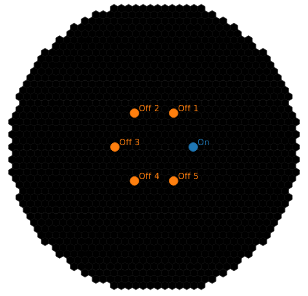
\includegraphics[width=0.8\textwidth]{fact_pics/wobblemode.png}
  \caption{wobblem-mode of the FACT detector.}
  \label{fig:wobble}
\end{figure}

\subsection{datasamples}
The given datasamples are preprocessed based on the analysis chain typical for data from Cherenkov-Telescopes.
For the shower-events three attributes of the original partilces must be reconstructed: the particle class, the energy and the direction to the origin.
The particle class is typical a gammaray or a hadron for example a proton. The energy is reconstructed via regression and the direction to the origin is calculated with ad 2d regression also.
A typical event is shown in figure \ref{fig:event}.
\begin{figure}
  \centering
  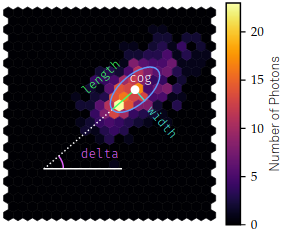
\includegraphics[width=0.8\textwidth]{fact_pics/event.png}
  \caption{a typical event. scale shows number of photons per bin.}
  \label{fig:event}
\end{figure}
The standard deviations \texttt{width} and \texttt{length} are calculated from a principal component analysis. The middle of the event is called \texttt{cog} and the orientation is defined through angle \texttt{delta} with regards to the x-axis.

The determination of the partcle class energye and direction of origin as well as detector acceptance complex simulations are necessary to generate training data.
\texttt{CORSIKA} was used to generate airshower, cherenkov-production and also particle propagation and finally saves the Cherenkov-light reaching the detector.
To simulate the FACT telescope \texttt{CERES} was used. Via machine learning, three datasamples were generated:
\begin{itemize}
  \item gammas from point-like source, observed with wobble mode
  \item gammas coming from random directions
  \item protons coming from random directions
\end{itemize}

\subsection{unfolding}
in physical measurements, the interessting parameters are never measured directly. In the astrophysics department energydepositions are used to yield the original attributes of the particles. This is called an "inverse problem" and can be described by
\begin{equation}
  g(y) = \int A(y,x) f(x) \symup{d}x + b(y)
  \label{eqn:convo}
\end{equation}
f(x) is the probability density function we want to know, depending on the physical parameter x. g(y) is the probability density function of the measured parameter y and b(y) is the background. A(y,x) is the concolution core represented by the detector.
To solve this problem, unfolding tecniques are used.
In a discrete form, equation \eqref{eqn:convo} can be written as
\begin{equation}
  \symbf{g} = \symbf{A}\symbf{f} + \symbf{b}
\end{equation}
Here, $\symbf{g}$ is the histogram of the estimated gamma-energies, $\symbf{f}$ is the histogram of the true gamma-energies.
$\symbf{A}$ is the migrationmatrixconstructed from the estimated and true gamma energies and $\symbf{b}$ is the background derived from the off-regions.

\subsubsection{naive SVD unfolding}
First the pseudoinverse matrix $A^{+}$ for non-quadratic matrices.
\begin{equation}
  \hat{\symbf{f}} = \symbf{A}^{+}(\symbf{g} - \symbf{b})
\end{equation}
This equation is equivalent to the least-square methode

\subsubsection{poisson-likelihood-unfolding}
When $\symbf{g}$ follows a poisson distribution a maximum-likelihood fit can be performed.
The probability to measure $g_i$ is
\begin{align}
  \symup{P}(g_i) &= \mathcal{P}(g_i, \lambda_i) \\
  \shortintertext{with}
  \symbf{\lambda} &= \symbf{A}\symbf{f} + \symbf{b} \\
  \intertext{minimizing the negative log-likelihood yields}
  -\ln(\mathcal{L}) &= \sum_{i=1}^{M} = -g_i \ln(\lambda_i) + \lambda_i \\
  \intertext{the estimator for $\symbf{f}$ is then}
  \hat{\symbf{f}} &= \text{argmin}(-\ln(\mathcal{L}(\symbf{f}|\symbf{A},\symbf{g},\symbf{b})))
\end{align}
